The differential operator
\[
Lu=
x^2\frac{\partial^2u}{\partial x^2}
+xy\frac{\partial^2u}{\partial x\partial y}
+y^2\frac{\partial^2u}{\partial y^2}
+3x^2y^2u.
\]
is defined on the domain
\[
\Omega=\{
(x,y)\,|\,\pi < xy < 2\pi, x < \pi,y < \pi
\}.
\]
\begin{teilaufgaben}
\item
Draw the domain $\Omega$.
\item
Is $L$ elliptic, hyperbolic or parabolic?
\item
Show that the function $u(x,y)=\sin(xy)$ is a solution of the differential
equation
\[
Lu=xy\cos(xy)
\]
on the domain $\Omega$ with boundary values
\begin{align*}
u(x,y)&=0            &&\text{$xy=\pi$ or $xy=2\pi$},\\
u(\pi,y)&=\sin(\pi y)&&1\le y\le 2,\\
u(x,\pi)&=\sin(\pi x)&&1\le x\le 2.
\end{align*}
\item
Why is this the only solution in the part of the domain where
$x>0$, $y>0$?
\end{teilaufgaben}

\begin{loesung}
\begin{teilaufgaben}
\item
The domain in the first quadrant is bounded by two hyperbolas and
two straight line segments:
\begin{center}
\includeagraphics[width=0.6\hsize]{bild-1}
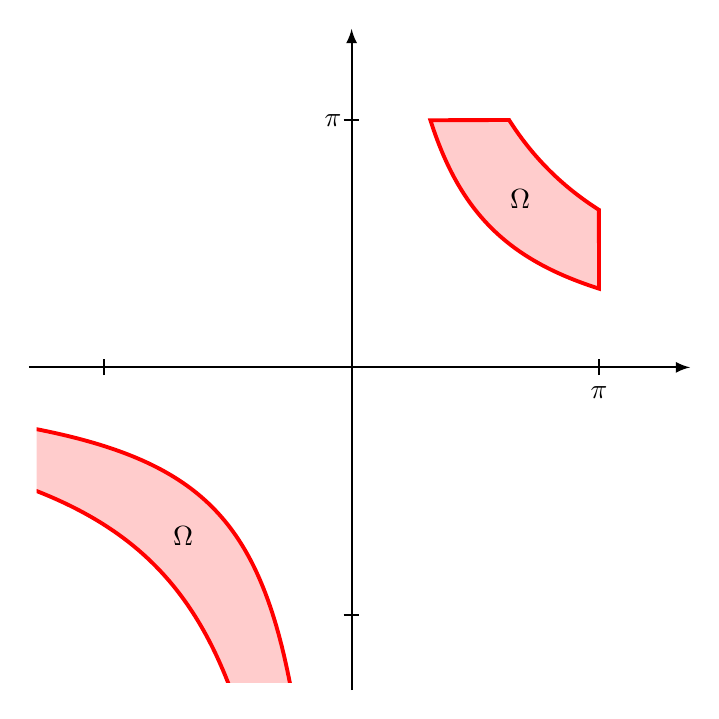
\begin{tikzpicture}[>=latex,thick]
\pgfmathparse{sqrt(3.1415)*(1+sqrt(2))/2}
\xdef\u{\pgfmathresult}
\begin{scope}
\clip (-4,-4) rectangle (0,0);
\fill[color=red!20]
	plot[domain=-4.2:{-3.1415/4.2},samples=100] (\x,{3.1415/\x})
	--
	plot[domain={-2*3.1415/4.2}:-4.2,samples=100] (\x,{2*3.1415/\x})
	--
	cycle;
\draw[color=red,line width=1.4pt]
	plot[domain=-4.2:{-3.1415/4.2},samples=100] (\x,{3.1415/\x});
\draw[color=red,line width=1.4pt]
	plot[domain=-4.2:{-2*3.1415/4.2},samples=100] (\x,{2*3.1415/\x});
\end{scope}
\begin{scope}
\fill[color=red!20]
	plot[domain=3.1415:1,samples=100] (\x,{3.1415/\x})
	--
	plot[domain=2:3.1415,samples=100] (\x,{2*3.1415/\x})
	-- cycle;
\draw[color=red,line width=1.4pt]
	plot[domain=3.1415:1,samples=100] (\x,{3.1415/\x})
	--
	plot[domain=2:3.1415,samples=100] (\x,{2*3.1415/\x})
	-- cycle;
\end{scope}
\node at (\u,\u) {$\Omega$};
\node at (-\u,-\u) {$\Omega$};
\draw[->] (-4.1,0) -- (4.3,0);
\draw[->] (0,-4.1) -- (0,4.3);
\draw (3.1415,-0.1) -- (3.1415,0.1);
\draw (-3.1415,-0.1) -- (-3.1415,0.1);
\draw (-0.1,3.1415) -- (0.1,3.1415);
\draw (-0.1,-3.1415) -- (0.1,-3.1415);
\node at (3.1415,0) [below] {$\pi\mathstrut$};
\node at (0,3.1415) [left] {$\pi\mathstrut$};
\end{tikzpicture}
\end{center}
However, there is another part in the third quadrant, not connected to
the part in the first quadrant.
The part of the domain in the third quadrant is unbounded, the entire
area between the hyperbolas belongs to that part.
\item
The symbol matrix is
\[
A=\begin{pmatrix}
x^2&\frac12xy\\
\frac12xy&y^2
\end{pmatrix}
\]
To decide whether the two eigenvalues have the same sign, it is sufficient
to compute the determinant:
\[
\det(A)=x^2y^2-\frac14x^2y^2=\frac34x^2y^2>0,
\]
so the operator is elliptic.
\item
We have to check whether the differential equation is satisfied and 
whether the boundary conditions hold.
The partial derivatives are
\begin{align*}
\frac{\partial u}{\partial x}&=y\cos(xy)
&
\frac{\partial^2 u}{\partial x^2}&=-y^2\sin(xy)
\\
&&\frac{\partial^2 u}{\partial x\partial y}&=\cos(xy)-xy\sin(xy)
\\
\frac{\partial u}{\partial y}&=x\cos(xy)
&
\frac{\partial^2 u}{\partial y^2}&=-x^2\sin(xy)
\end{align*}
This turns the differential equation into
\begin{align*}
Lu&=-x^2y^2\sin(xy)+xy(\cos(xy)-xy\sin(xy))-x^2y^2\sin(xy)+3x^2y^2\sin(xy)\
\\
&=xy\cos(xy),
\end{align*}
so it holds true.
The boundary conditions along the curved parts of the boundary are
\begin{align*}
xy&=\pi&\Rightarrow\quad u(x,y)&=\sin(xy)=\sin\pi=0\\
xy&=2\pi&\Rightarrow\quad u(x,y)&=\sin(xy)=\sin2\pi=0,
\end{align*}
along the straight line segments they are
\begin{align*}
u(\pi,y)&=\sin(\pi y)
&u(x,\pi)&=\sin(x\pi),
\end{align*}
so the boundary conditions also hold.
Thus $u$ is a solution of the partial differential equation.
\item
The solution of an elliptic partial differential equation is subject to
the maximum principle.
Another solution $\bar u(x,y)$ of the equation would lead to
$v=u-\bar u$ satisfying $Lu=0$, where $v$ vanishes on the boundary.
But since $v$ would need to have the maximum on the boundary, we 
conclude that $v=0$ or $u=\bar{u}$.
Thus there cannot be another solution.

But this argument only works for bounded domains, as e.~g.~the part of
$\Omega$ in the first quadrant.
So the solution there actually is unique.
For the domain in the third quadrant there may be additional solutions.
\qedhere
\end{teilaufgaben}
\end{loesung}
